\section{Virtualizzazione}\label{virtualizzazione}

È l'astrazione dei componenti hardware di elaboratori per renderli
disponibili, come risorsa virtuale, al software.

In questo modo è possibile installare S.O. su hardware virtuale,
l\textquotesingle insieme di questo hardware è detto Virtual Machine.

\subsection{Vantaggi}\label{vantaggi}

\begin{itemize}
\item
  Utilizzo superiore dell'hardware;
\item
  Riduzione consumi e spazio;
\item
  Isolamento sistemi;
\item
  Più S.O. nello stesso hardware;
\item
  Gestione, portabilità e scalabilità migliore.
\end{itemize}

\subsection{Terminologia}\label{terminologia}

\begin{itemize}
\item
  \emph{Host}: macchina fisica dove gira il S.O. principale, dove si
  ospitano le macchine virtuali;
\item
  \emph{Guest}: è la macchina virtuale, si trova ``sopra'' l'host;
\item
  \emph{Hypervisor}: detto anche virtual machine monitor è quel software
  che avvia e crea le VM.
\end{itemize}

\subsection{Tipi di virtualizzazione}\label{tipi-di-virtualizzazione}

\begin{itemize}
\item
  \emph{Virt. Desktop}: l'utente crea una macchina virtuale sulla
  propria macchina fisica tramite un hypervisor di tipo 2 (hosted), per
  accedere alla VM l'utente utilizza le periferiche della propria
  macchina fisica. Utile per utilizzare software non compatibile sulla
  propria macchina;
\item
  \emph{Virt. Server}: si realizza una VM in un data center tramite S.O.
  dedicati e hypervisor di tipo 1 (bare-metal) permettendo di eseguire
  altri S.O. direttamente sull'hardware, l'utente ci accedere da remoto;
\item
  \emph{{[}...{]} CPU}: dobbiamo distinguere fra:
\end{itemize}

\begin{enumerate}
\def\labelenumi{\arabic{enumi}.}
\item
  \ul{Virtualizzazione}: si crea una CPU virtuale che esegue lo stesso
  tipo di istruzioni macchina della CPU reale. La CPU virtuale quindi
  può fare eseguire le istruzioni dei programmi direttamente dalla CPU
  reale;
\item
  \ul{Emulazione}: si costruisce una CPU virtuale che esegue istruzioni
  di tipo diverso da quello della CPU reale, quindi le istruzioni devono
  essere tradotte in istruzioni macchina.
\end{enumerate}

\subsection{Protection Ring}\label{protection-ring}

Sono 4 ``anelli'' di protezione per le CPU moderne, vanno da 0 a 3
quando la CPU è settata per stare nei rings di livello più alto è
abilitata a fare istruzioni non privilegiate.

\ul{Nei rings più bassi} la CPU può fare tutte quelle \ul{istruzioni più
pericolose} tipiche del S.O.

\subsection{Virt. livello HW}\label{virt.-livello-hw}

Sono le VM e all\textquotesingle utente del sistema di virtualizzazione
viene presentata un\textquotesingle interfaccia su cui installare un
sistema operativo, quindi una CPU virtuale (ma dello stesso tipo della
CPU fisica) e risorse HW virtuali.

I S.O. vengono eseguiti in modo concorrente sullo stesso hardware e
possono solitamente essere eterogenei e l'hypervisor multiplexa
l'accesso alle risorse.

In questa categoria può capitare che l'hypervisor possa svolgere il
ruolo di S.O. essendo un processo all'interno di un altro S.O.

\subsubsection{Virt. tipo 1 e 2}\label{virt.-tipo-1-e-2}

La virtualizzazione di tipo 1 o \emph{\textbf{bare-metal}} è quando il
s.o. host è assente e l'hypervisor prende il suo posto (virtualizzazione
server).

La virtualizzazione di tipo 2 o \emph{\textbf{hosted}} è quando un
hypervisor è un processo utente (virtualizzazione desktop).

\subsubsection{Full e Para
Virtualization}\label{full-e-para-virtualization}

È una suddivisione della virtualizzazione HW:

\begin{itemize}
\item
  \textbf{Para-virtualization}: la VM presenta
  un\textquotesingle interfaccia differente rispetto ad una macchina
  fisica. Questo comporta dover modificare il sistema operativo guest
  per consentire l\textquotesingle esecuzione
  all\textquotesingle interno della macchina virtuale stessa. Si
  utilizzano API (\emph{hypercall}) per permettere al s.o. guest di
  interfacciarsi e permettere tutte le operazioni classiche di un
  sistema.
\item
  \textbf{Full-virtualization}: le macchine virtuali hanno la stessa
  interfaccia di una fisica, il sistema guest non sa di essere virtuale
  e non c'è bisogno di modificare il s.o.
\end{itemize}

\begin{quote}
Per eseguire le istruzioni privilegiate, limitando e controllando le
azioni in modo da evitare problemi, vengono adottate due modalità:
\end{quote}

\begin{enumerate}
\def\labelenumi{\arabic{enumi}.}
\item
  \textbf{Binary translation}: consiste nel scrivere le istruzioni
  binarie. La CPU opera in modalità debug, ad ogni comando sospende
  l'esecuzione, analizza il codice e copia delle parti in una cache dove
  viene modificato per far in modo che il codice lavori sulle risorse
  della VM.
\item
  \textbf{Hardware assisted}: viene aggiunto un nuovo ring chiamato
  \emph{ring -1}, il sistema host e l'hypervisor vengono eseguiti in
  quest'ultimo ring mentre il guest in quello 0.
\end{enumerate}

\begin{quote}
Così facendo il sistema operativo guest può eseguire le istruzioni
privilegiate, sotto però il controllo dell\textquotesingle hypervisor.
\ul{È possibile annidare più VM una dentro l'altra} essendoci più
tabelle con le info su ciascuna VM.

Nella para-virtualization questo problema non persiste perchè il s.o.
non invoca direttamente le istruzioni privilegiate.
\end{quote}

\subsection{Virt. livello OS}\label{virt.-livello-os}

Sono i container, all\textquotesingle utente viene presentata una
partizione del sistema operativo corrente, su cui installare ed eseguire
applicazioni che \emph{rimangono isolate} nella partizione, \emph{pur
accedendo ai servizi di uno stesso o.s}.

In questo tipo la virtualizzazione è composta da un solo kernel e
istanze isolate che possono essere modificate e utilizzate
indipendentemente tra loro.

\subsection{Container}\label{container}

Creano uno spazio utente isolato (anche se non perfetto), con proprie
librerie e file, isolando una applicazione dal resto del sistema
operativo, più container possono appoggiarsi ad uno stesso spazio kernel
e usano servizi di uno stesso S.O.

Il container offre basso sovraccarico per il content-switching e di
memoria senza la possibilità di usare S.O. differenti.

I principali container sono:

\begin{itemize}
\item
  \textbf{Docker}: si appoggia sul s.o. Linux che fornisce un supporto
  per container detto LXC (Linux Container);
\item
  \textbf{Hyper-V}: proprietario di Microsoft, in realtà si chiamano
  container ma sono delle semplici macchine virtuali;
\item
  \textbf{Container di Windows Server}: sono effettivamente dei
  container.
\end{itemize}

\subsubsection{Docker Swarm}\label{docker-swarm}

Distribuire il carico su più container e su più macchine.

In Docker Swarm esiste un cluster di macchine comandate da un
\textbf{nodo Manager} (gli altri nodi sono detti \emph{worker}), il
\textbf{nodo Manager} distribuisce gli \ul{insiemi} (service) e i
\ul{container} (task) fra i \emph{worker}; i task e i service insieme
formano una applicazione.


\includegraphics[width=6.26772in,height=2.875in]{media/image3.png}

\subsubsection{Kubernetes}\label{kubernetes}

Fornisce automaticamente scalabilità e resilienza ad applicazioni basate
su container docker, in esecuzione su cluster di host fisici o virtuali.

Le applicazioni progettate per kubernetes sono costituite da più pods,
dove ciascun pods è un insieme di container che cooperano e comunicano
tra loro come se si trovassero in un unico host fisico e svolgono un
servizio; un pod può realizzare un servizio web mentre un altro può
eseguire una serie di calcoli.

Un pod è replicabile su più istanze e le istanze possono essere eseguite
su host diversi, in questo caso l'insieme degli host (fisici o virtuali)
è detto nodi di cluster, un host svolge il ruolo di controllore (control
plane o controllore del cluster) degli host e dei pod e si interfaccia
con l'esterno.

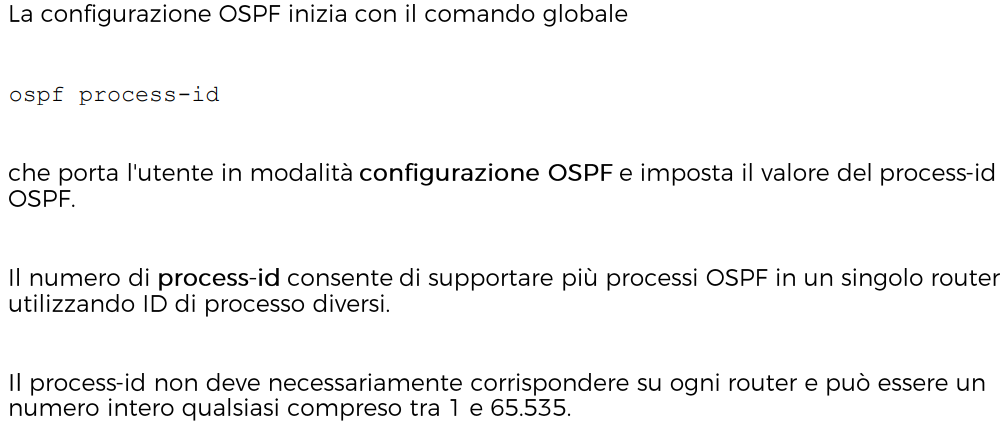
\includegraphics[width=6.26772in,height=1.43056in]{media/image4.png}


\includegraphics[width=6.26772in,height=1.75in]{media/image5.png}

All'aumento del carico l'applicazione può configurare Kubernetes
affinchè faccia 3 operazioni:

\begin{enumerate}
\def\labelenumi{\arabic{enumi}.}
\item
  \textbf{Autoscaling verticale}: aumento le risorse (CPU, RAM,...) di
  un pod;
\item
  \textbf{Autoscaling orizzontale}: aumento repliche dei pods
  applicativi;
\item
  \textbf{Cluster autoscaling:} aumento dei nodi che compongono il
  cluster ridistribuendo i pods.
\end{enumerate}

Per realizzare questi autoscaling su host fisici occorre un sistema di
accensione host guidabile via software, per gli host virtuali occorre un
supporto che ci dia la possibilità di creare e configurare nuove VM in
automatico via software

E\textquotesingle{} possibile creare un cluster kubernetes formato da
host che siano macchine virtuali, create manualmente su host fisici
oppure possono essere create via software (OpenSpace) su cloud pubblici
o privati.

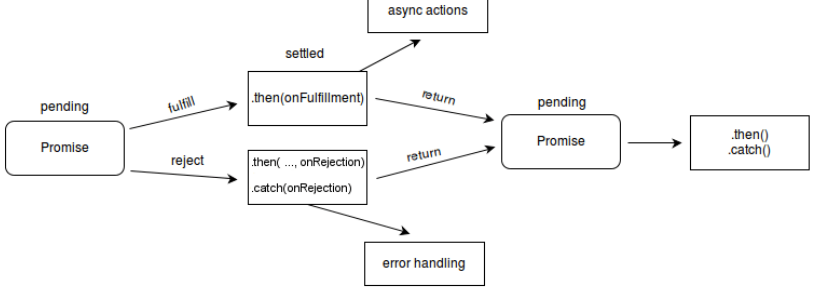
\includegraphics[width=6.26772in,height=2.79167in]{media/image7.png}

\subsubsection{Kubernetes-as-a-Service}\label{kubernetes-as-a-service}

Alcuni sistemi cloud offrono un servizio kubernetes senza che sia
necessario creare esplicitamente il cluster kubernetes, il cluster viene
creato ed installato dal provider cloud su richiesta e a chi produce
l\textquotesingle applicazione vengono fornite delle API mediante le
quali chiedere di inizializzare il cluster kubernetes e di dispiegarsi
sopra l\textquotesingle applicazione organizzata per kubernetes; queste
API però sono diverse fra servizi cloud.

\subsubsection{Container-as-a-Service}\label{container-as-a-service}

I sistemi cloud permettono di far eseguire un container, la cui immagine
è fornita dallo sviluppatore dell\textquotesingle applicazione, in
molteplici istanze su un cluster kubernetes-as-a-service costruito
nascostamente dal provider stesso.

Il container viene incapsulato in un pod predisposto dal provider cloud
ed eseguito nel cluster kubernetes.

\section{DOCKER}\label{docker}

\subsection{Info generali}\label{info-generali}

Esistono tre componenti essenziali:

\begin{itemize}
\item
  \textbf{Docker Engine}: si interfaccia con Linux e utilizza API per
  lavorare con il ciclo di vita dei containers {[} \emph{provides the
  core capabilities of managing containers} {]};
\item
  \textbf{Docker Tools}: insieme di funzioni a linea di comando che
  permettono di parlare con le API esposte dal componente
  precedentemente citato. Comandi utili per far partire container,
  creare loro immagini e configurare memoria e reti;
\item
  \textbf{Docker Registry}: dove le immagini dei container sono salvate
  con tags e versioni differenti.
\end{itemize}

\begin{quote}
\emph{docker info =\textgreater{} mostra i dettagli del Docker Engine}

\emph{docker version=\textgreater{} mostra i dettagli del Docker Tools
(+ Engine)}
\end{quote}

\subsection{Installazione}\label{installazione}

\emph{Prima di procedere si necessita un s.o. LUbuntu e un account
Docker Hub.}

\begin{enumerate}
\def\labelenumi{\arabic{enumi}.}
\item
  Installare curl: sudo apt-get update
\end{enumerate}

sudo apt-get install curl

\begin{enumerate}
\def\labelenumi{\arabic{enumi}.}
\setcounter{enumi}{1}
\item
  Installare docker engine: curl -fsSL https://get.docker.com -o
  get-docker.sh
\end{enumerate}

\begin{quote}
sudo sh get-docker.sh
\end{quote}

\begin{enumerate}
\def\labelenumi{\arabic{enumi}.}
\setcounter{enumi}{2}
\item
  Aggiungere l'utente in uso fra i sudoers {[}evitando di dover usare
  sempre sudo prima dei comandi{]}: sudo usermod -aG docker \$\{USER\}
\end{enumerate}

\begin{quote}
id -nG {[}controllo lista sudoers{]}

su - \$\{USER\} {[}Ricarico utente{]}
\end{quote}

\subsection{Comandi Docker}\label{comandi-docker}

Sintassi generale: \emph{\textbf{docker {[}option{]} {[}command{]}
{[}arguments{]}}}

Usando il comando: `docker' posso controllare tutti i sottocomandi.

\subsection{Docker images e container}\label{docker-images-e-container}

I container docker sono creati tramite immagini docker che normalmente
vengono prese da Docker Hub, un portale dove tutti possono condividere
le proprie immagini Docker; per scaricare queste immagini usiamo il
comando:

``\emph{\textbf{docker run {[}images name{]}}}''.

Il comando cerca prima l'immagine in locale e se non la trova la
scarica, poi Docker crea un container dall'immagine ed esegue
l'applicazione al suo interno; l'immagine è copiata in uno spazio
locale.

Con il seguente comando invece otteniamo la possibilità di interagire
con il container tramite shell:

``\emph{\textbf{docker run -it {[}images name{]}}}''.

Se inseriamo, dopo `-it', anche \emph{\textbf{- -name}} seguito da una
stringa daremo un un nome custom al container.

\subsubsection{Ricerca e Download}\label{ricerca-e-download}

Per cercare immagini su Docker Hub si usa:

``\emph{\textbf{docker search {[}images name{]}}}''.

Il ritorno del comando sarà una lista delle immagini con il nome
combacia con quello inserito nel comando (le immagini ufficiali avranno
il flag \emph{{[}OK{]}} sotto la voce OFFICIAL) per scaricare:

``\emph{\textbf{docker pull {[}images name{]}}}''.

\subsubsection{Eliminazione}\label{eliminazione}

Per rimuovere le immagini scaricate si usa il comando:

``\emph{\textbf{docker rmi {[}images name1{]} {[}images name2{]}
{[}images name N{]}}}''.

Per rimuovere i container si usa il comando:

``\emph{\textbf{docker rm {[}container name{]} or {[}container
ID{]}}}''.

\subsubsection{Lavorare dentro i
container}\label{lavorare-dentro-i-container}

Inserendo `\emph{\textbf{-it}}' (come visto prima) nel comando run
potremmo inserire comandi dentro il container e quindi usare la shell
per fare operazioni dentro di esso.

\ul{In questo caso non è necessario il prefisso sudo}

\subsubsection{Gestione}\label{gestione}

Per la gestione dei container esistono diversi comandi:

\begin{itemize}
\item
  \emph{\textbf{docker ps}} =\textgreater{} mostra i container attivi,
  con ` \emph{\textbf{-a}} ' alla fine del comando possiamo visionare
  anche quelli inattivi (inserendo `\emph{\textbf{-q}}' mostriamo solo
  gli ID);
\item
  \emph{\textbf{docker ps -l}} =\textgreater{} mostra i container più
  recente;
\item
  \emph{\textbf{docker stop {[}container name{]} or {[}container ID{]}}}
  =\textgreater{} ferma i container in esecuzione;
\item
  \emph{\textbf{docker start {[}container name{]} or {[}container
  ID{]}}} =\textgreater{} fa ripartire un container, con `
  \emph{\textbf{-ia}} ` dopo lo start possiamo usare i canali STDIN e
  STDOUT.
\item
  \emph{\textbf{docker commit {[}container ID{]} {[}new image name{]}}}
  =\textgreater{} salva lo stato del container in una nuova immagine
\end{itemize}

\subsection{Networks}\label{networks}

Quando creo un container in automatico viene creata
un\textquotesingle interfaccia di rete del container; oppure è possibile
indicare quale tipo di interfaccia di rete vogliamo mettere nel
container (dipendono dal tipo di driver).

Per funzionare è necessario avere dei driver specifici, alcuni già
presenti sono:

\begin{itemize}
\item
  \emph{\textbf{bridge}}: inserito di default in ogni container,
  consente di comunicare con l\textquotesingle host e comunicare con
  l\textquotesingle esterno\emph{;}
\item
  \emph{\textbf{host}}: consente ad un container di utilizzare
  l\textquotesingle interfaccia di rete della macchina host come se
  fossero sue, però così facendo vado a perdere
  l\textquotesingle isolamento del container verso
  l\textquotesingle esterno;
\item
  \emph{\textbf{overlay}}: connette più Docker deamons insieme e
  permette di comunicare fra loro\emph{;}
\item
  \emph{\textbf{macvlan}}: permette di assegnare un indirizzo MAC ad un
  container, rendendolo agli occhi di tutti un device fisico (utile per
  lavorare con le legacy application che si aspettano di essere connesse
  ad una rete fisica)\emph{;}
\item
  \emph{\textbf{none}}: disabilita tutti i networking\emph{;}
\item
  \emph{\textbf{custom network plugins}}.
\end{itemize}

\begin{quote}
\emph{- -networks =\textgreater{} per assegnare uno di questi driver ad
un container}
\end{quote}

Un \emph{bridge network} permette ai container connessi allo stesso
bridge di comunicare, isolando coloro non connessi.

Le \emph{docker embedded DNS server} permettono la risoluzione dei nomi
per container connessi alla stessa network.

\subsection{Compose}\label{compose}

Docker compose serve per scrivere un documento di tipo YML per creare

delle applicazioni costituite da più container; lo strumento originario
si

chiama docker-compose ed è un comando installato separatamente rispetto
a

docker.

\subsection{DockerFile}\label{dockerfile}

È uno script che contiene un'insieme di comandi e istruzioni che vengono
eseguite automaticamente nell'ambiente di docker per creare nuove
immagini; sotto si elencano alcuni di questi comandi.

\subsubsection{Comandi}\label{comandi}

\begin{itemize}
\item
  \textbf{FROM} =\textgreater{} indica l'immagine da dove bisogna creare
  un'immagine tutta nuova;
\item
  \textbf{MAINTAINER} =\textgreater{} contiene il nome di chi
  ``mantiene'' l'immagine;
\item
  \textbf{RUN} =\textgreater{} esegue un comando durante la build;
\item
  \textbf{COPY} =\textgreater{} copia un file dall'host alla nuova
  immagine;
\item
  \textbf{ADD} =\textgreater{} come il precedente ma è possibile mettere
  anche un URL come sorgente;
\item
  \textbf{ENV} =\textgreater{} definisce una variabile di ambiente
  utilizzabile in altri ambienti;
\item
  \textbf{CMD} =\textgreater{} esegue un comando quando si costruisce un
  nuovo container dall'immagine docker;
\item
  \textbf{ENTRYPOINT} =\textgreater{} il comando di default da fare
  quando il container è in esecuzione;
\item
  \textbf{WORKDIR} =\textgreater{} indica dove fare i comandi fatti con
  `CMD';
\item
  \textbf{USER} =\textgreater{} ;
\item
  \textbf{VOLUME} =\textgreater{} ;
\end{itemize}

\subsection{Docker Swarm}\label{docker-swarm-1}

Permette di utilizzare un'applicazione fatta da container su più
macchine (fisiche o virtuali), l\textquotesingle insieme di macchine (o
nodi) si chiama SWARM, dove un nodo che prende il nome di manager
gestisce l'insieme.

\emph{docker swarm init =\textgreater{} per scegliere il manager}

Lo swarm può lanciare degli stack (gruppo di servizi), dove ogni
servizio è lo stesso visto nel Compose ( un'immagine di container e le
proprie strutture). Ogni stack è composto da tanti task (ogni istanza di
un container) e il manager gestisce le richieste fra task.

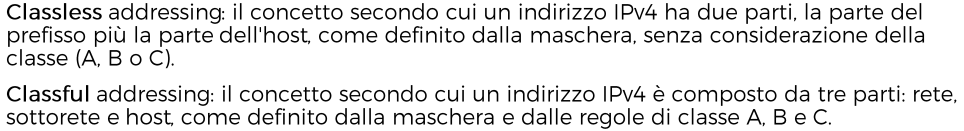
\includegraphics[width=6.26772in,height=3.02778in]{media/image6.png}

\emph{In essence, a stack is a set of tasks (working containers),
grouped in services, running over a cluster of worker nodes and
coordinated by a manager node.}

\subsection{Kubernetes}\label{kubernetes-1}

Kubernetes è un\textquotesingle architettura software con una struttura
client-server che esegue su un cluster (cioè un gruppo di host) una
applicazione.

L\textquotesingle interfacciamento dell\textquotesingle amministratore
di kubernetes avviene tipicamente mediante un client.

Si può gestire bene la scalabilità dell'applicazione e rispetto a swarm
c'è una organizzazione maggiore fra container grazie ai \textbf{pods}.

I pods sono un' insieme di più container con caratteristiche simili
(stessi indirizzi ip, stesso spazio di porte) che comunicano fra loro
come se fossero sulla stessa macchina fisica.

Un insieme di istanze dello stesso pod (repliche) è detto deployments.

I pods sono classificati con \textbf{label}, stringhe di nomi + valori,
ugual label ugual funzionalità.

Per ricercare una risorsa invece si utilizza il \textbf{selectors},
andando a specificare una determinata label.

\subsubsection{Services}\label{services}

Un servizio è un insieme di pods individuati da un selettore, il
servizio tipicamente include anche la politica con cui viene effettuato
il bilanciamento di carico delle richieste tra i diversi pods di quello
stesso servizio.

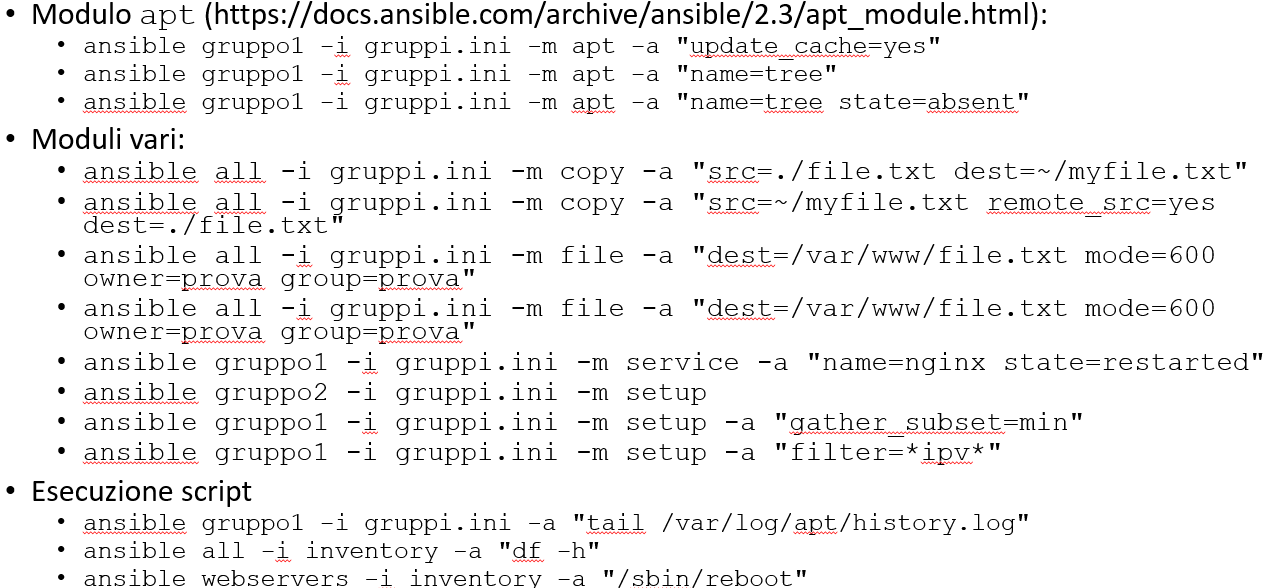
\includegraphics[width=6.26772in,height=2.04167in]{media/image2.png}

\subsubsection{Autoscaling}\label{autoscaling}

Tecnica che incrementa e/o riduce in modo dinamico l'ammontare di
risorse a disposizione di una o più server farm.

In kubernetes si utilizza quando all'aumentare di richieste per dei
servizi si necessita di più pod.

\section{BASH}\label{bash}

\subsection{Permessi}\label{permessi}

Ogni file ha un proprietario ed un gruppo del proprietario, il
proprietario/creatore poi può cambiare il proprietario del file con il
comando:

\emph{\textbf{chown {[}nuovoProprietario{]} {[}nomeFile{]}}}

il gruppo:

\emph{\textbf{chgrp {[}nuovoGruppo{]} {[}nomeFile{]}}}

i premessi::

\emph{\textbf{chmod {[}numeriDeiPermessi{]} {[}nomeFile{]}}}

Ciascun file mantiene diversi diritti di lettura, scrittura ed
esecuzione assegnati al proprietario, al gruppo del proprietario e a
tutti gli altri:

\begin{itemize}
\item
  Lettura (valore 4, simbolo r);
\item
  Scrittura (valore 2, simbolo w);
\item
  Esecuzione (valore 1, simbolo x);
\end{itemize}

Quindi se voglio, per esempio, mettere che tutti possono fare tutto su
quel file devo fare:

\emph{\textbf{chmod 777 {[}nomeFile{]}}}

questo perché il 1° sette indica scrittura, lettura e esecuzione
all'user (4+2+1), il 2° sette indica gli stessi permessi al gruppo e il
3° sette indica i permessi di tutti gli altri.


\includegraphics[width=6.26772in,height=1.01389in]{media/image1.png}

\subsection{Caratteri con utilizzi
speciali}\label{caratteri-con-utilizzi-speciali}

\begin{itemize}
\item
  \textbf{;} ➡ separatore tra comandi , che stabilisce cioè dove finisce
  un comando e dove inizia il successivo;
\item
  \textbf{\textbackslash{}} ➡ carattere di escape, ferma
  l'interpretazione di alcuni caratteri speciali;
\item
  \textbf{``...''} ➡ tutto ciò che è scritto al suo interno viene letto
  in maniera letterale;
\item
  \textbf{* ? {[}\ldots{]}} ➡ sono caratteri che vengono inseriti
  dall'utente nei comandi digitati e che la shell interpreta cercando di
  sostituirli con una sequenza di caratteri; possono essere sostituiti
  con:
\end{itemize}

\begin{enumerate}
\def\labelenumi{\arabic{enumi}.}
\item
  * :una qualunque sequenza di caratteri;
\item
  ? :un solo e unico carattere;
\item
  {[}...{]} :un solo carattere tra quelli specificati in un elenco
  scritto all'interno dei caratteri.
\end{enumerate}

\begin{itemize}
\item
  \textbf{\textless{}} ➡ riceve input da file;
\item
  \textbf{\textgreater{}} ➡ mandare std output verso file eliminando il
  vecchio contenuto del file;
\item
  \textbf{\textgreater\textgreater{}} ➡ mandare std output verso file
  aggiungendolo al vecchio contenuto del file;
\item
  \textbf{\textbar{}} ➡ redirige l\textquotesingle output di un
  programma nell' input di un altro programma;
\item
  \textbf{\textless\textless{}}\emph{parolaFine} ➡ redirige tutto da
  dopo il metacarattere alla prossima apparizione della keyword
  \emph{parolaFine};
\item
  \textbf{\textless\textless\textless{}}\emph{parolaFine} ➡ viene
  ridirezionato nell\textquotesingle input la parola che compare subito
  dopo il metacarattere;
\item
\end{itemize}

\subsection{Esecuzione script}\label{esecuzione-script}

Normalmente, se una shell lancia uno script, questo viene eseguito in
una subshell e le modifiche fatte su variabili non vengono viste dal
padre.

È possibile però che una shell possa eseguire uno script senza creazione
di subshell, per farlo basta usare il comando:

\emph{\textbf{source} nomeScript}

\textbf{oppure}

\emph{\textbf{.} nomeScript}

Se però invochiamo con source uno script \emph{che necessita} di un
\ul{interprete diverso} provochiamo dei problemi, poiché \emph{non verrà
lanciato l\textquotesingle interprete corretto} indicato nella prima
riga dello script.

\subsection{Comandi}\label{comandi-1}

\subsubsection{Set}\label{set}

Se il comando viene lanciato \textbf{senza parametri} \emph{visualizza
tutte le variabili della shell}, altrimenti lanciato \textbf{con
parametri} serve a \emph{settare o resettare un\textquotesingle opzione
di comportamento della shell} in cui viene lanciato.

\subsubsection{Echo}\label{echo}

Stampa quello che si scrive dopo il comando.

\subsubsection{Mkdir/Rmdir}\label{mkdirrmdir}

Crea/elimina una directory nel percorso specificato.

\subsubsection{Cat}\label{cat}

Visualizza in output il contenuto del file specificato.

\subsubsection{Env}\label{env}

Visualizza tutte le variabili e i loro valori.

\subsubsection{Which}\label{which}

Visualizza il percorso in cui si trova (solo se nella PATH)
l'eseguibile.

\subsubsection{Sed}\label{sed}

Il comando è così strutturato:

\emph{\textbf{sed} `\textbf{s}/es1/es2/\textbf{g}' nomeFile}

In questo modo per ogni riga processata (senza \textbf{g} solo la prima)
\emph{es1} verrà sostituito con \emph{es2}.

\section{DOMANDE}\label{domande}

\subsection{Parte 1}\label{parte-1}

\begin{enumerate}
\def\labelenumi{\arabic{enumi}.}
\item
  Un container in ambiente linux in cui esegue un web server, può essere
  considerato un "micro-servizio"?. Motivare la risposta.
\end{enumerate}

\begin{quote}
Si, un container Linux che ospita un web server può rappresentare uno
dei microservizi di un\textquotesingle applicazione più ampia
\end{quote}

\begin{enumerate}
\def\labelenumi{\arabic{enumi}.}
\setcounter{enumi}{1}
\item
  Citare i due modi mediante i quali si risolve il problema delle
  istruzioni privilegiate nella full-virtualization.
\end{enumerate}

\begin{quote}
Per eseguire le istruzioni in kernel mode (ring 0) si usano le seguenti
tecniche:
\end{quote}

\begin{itemize}
\item
  Binary translation: si riscrivono a run-time le parti del codice del
  s.o.guest che dovrebbero essere eseguite in modo privilegiato.
\item
  Hardware assisted: viene aggiunto un nuovo ring chiamato \emph{ring
  -1}, il sistema host e l'hypervisor vengono eseguiti in quest'ultimo
  ring mentre il guest in quello 0 (esecuzione di istruzioni
  privilegiate sotto il controllo dell'hypervisor).
\end{itemize}

\begin{enumerate}
\def\labelenumi{\arabic{enumi}.}
\setcounter{enumi}{2}
\item
  In una macchina fisica in cui è installato Docker, a cosa serve il
  docker registry?
\end{enumerate}

\begin{quote}
Componente essenziale di un docker, è dove le immagini dei container
sono salvate con tags e versioni differenti.
\end{quote}

\begin{enumerate}
\def\labelenumi{\arabic{enumi}.}
\setcounter{enumi}{3}
\item
  Posso mettere in esecuzione due container, partendo dalla stessa
  immagine, in modo che i due container eseguano simultaneamente ?
  Potrebbero generarsi interferenza tra i due container? Motivare la
  risposta.
\end{enumerate}

\begin{quote}
È possibile eseguire due container dalla stessa immagine
contemporaneamente e non dovrebbero generarsi problemi essendo i
container creati per rimanere isolati e lavorare in autonomia.
\end{quote}

\begin{enumerate}
\def\labelenumi{\arabic{enumi}.}
\setcounter{enumi}{4}
\item
  Supponiamo che un immagine di un container contenga tutto il
  necessario per eseguire un applicativo, ad esempio il database
  documentale mongo. Però in quell\textquotesingle immagine non è
  installato un altro applicativo, ad esempio il magnifico editor
  testuale vim. L\textquotesingle applicativo vim è però installato nel
  sistema operativo Linux della macchina fisica. Supponiamo di mettere
  in esecuzione un container partendo da quell\textquotesingle immagine.
  Posso eseguire, all\textquotesingle interno del container,
  l\textquotesingle applicativo vi? Motivare la risposta
\end{enumerate}

\begin{quote}
Si, i container possono utilizzare gli stessi servizi del s.o. host.
\end{quote}

\begin{enumerate}
\def\labelenumi{\arabic{enumi}.}
\setcounter{enumi}{5}
\item
  A cosa serve il comando docker build ?
\end{enumerate}

Il comando docker build è utilizzato per creare
un\textquotesingle immagine Docker a partire

da un Dockerfile; permette di definire in modo dichiarativo tutte le

configurazioni e le dipendenze necessarie per
l\textquotesingle esecuzione dell\textquotesingle applicazione

all\textquotesingle interno del container.

\begin{enumerate}
\def\labelenumi{\arabic{enumi}.}
\setcounter{enumi}{6}
\item
  Posso salvare l\textquotesingle immagine di un container in
  esecuzione, dopo averlo stoppato? Se ritenete che si possa, quale
  comando dovreste usare?
\end{enumerate}

\begin{quote}
Si, dopo aver stoppato il container con \emph{\textbf{docker stop}}
possiamo salvare l'immagine in una nuova con \emph{\textbf{docker commit
{[}id container{]} {[}nuovo nome immagine{]}}}.
\end{quote}

\begin{enumerate}
\def\labelenumi{\arabic{enumi}.}
\setcounter{enumi}{7}
\item
  Che tipo di servizio offre il docker hub (https://hub.docker.com/) ?
\end{enumerate}

Docker Hub è un servizio di registro di container pubblico fornito da
Docker.

Offre una piattaforma centralizzata per la condivisione, la
distribuzione e la

collaborazione sulle immagini Docker.

\begin{enumerate}
\def\labelenumi{\arabic{enumi}.}
\setcounter{enumi}{8}
\item
  Un container offre un servizio sulla propria porta TCP 80. Nella
  macchina fisica in cui voglio eseguire il container, quella porta 80 è
  usata da un\textquotesingle altra applicazione. Senza modificare il
  container, posso eseguire quel container in modo da esporre il
  servizio offerto dal container su una diversa porta nella macchina
  fisica, ad esempio la porta 60000? Motivare la risposta.
\end{enumerate}

\begin{quote}
Sì è possibile, infatti il comando \emph{\textbf{docker run}} può
contenere tanti parametri, fra questi c'è il \emph{\textbf{-p}} che
permette di decidere in quale porta fisica (60000) deve essere mappata
la porta del container (80).
\end{quote}

\begin{enumerate}
\def\labelenumi{\arabic{enumi}.}
\setcounter{enumi}{9}
\item
  A cosa serve un Dockerfile ?
\end{enumerate}

È uno script che contiene un'insieme di comandi e istruzioni che vengono

eseguite automaticamente nell'ambiente di docker per creare nuove
immagini

\begin{enumerate}
\def\labelenumi{\arabic{enumi}.}
\setcounter{enumi}{10}
\item
  Quale è la principale funzionalità che viene messa a disposizione dal
  DNS embedded che docker automaticamente configura per i container che
  usano una stessa user-defined bridge network?
\end{enumerate}

\begin{quote}
Il DNS embedded permette la risoluzione dei nomi per container connessi
alla stessa network.
\end{quote}

\begin{enumerate}
\def\labelenumi{\arabic{enumi}.}
\setcounter{enumi}{11}
\item
  E\textquotesingle{} possibile attaccare un container a più di una
  rete?
\end{enumerate}

\begin{quote}
Sì, è possibile attaccare un container a quante reti si voglia basta che
usino differenti driver.
\end{quote}

\begin{enumerate}
\def\labelenumi{\arabic{enumi}.}
\setcounter{enumi}{12}
\item
  Che cos\textquotesingle è iptables/netfilter ?
\end{enumerate}

\begin{quote}
Iptables: è un comando (un eseguibile binario) che prende come argomenti

dei comandi con cui si definiscono delle regole che sono realizzate da
più

moduli del kernel linux;

Netfilter: è un insieme di moduli del kernel linux che lavorano su

pacchetti di rete.
\end{quote}

\begin{enumerate}
\def\labelenumi{\arabic{enumi}.}
\setcounter{enumi}{13}
\item
  Che cos\textquotesingle é docker-compose e a cosa serve ?
\end{enumerate}

\begin{quote}
È uno strumento che permette la creazione di applicazioni con più
container, la loro rimozione e il loro controllo in modo coordinato.
\end{quote}

\begin{enumerate}
\def\labelenumi{\arabic{enumi}.}
\setcounter{enumi}{14}
\item
  Nel contesto di docker swarm, qual\textquotesingle è la differenza tra
  un nodo manager ed un nodo worker?
\end{enumerate}

\begin{quote}
il nodo manager oltre a gestire gli altri nodi (worker) e distribuire i
task fra loro riceve anche le richieste dai client esterni e le
distribuisce ai vari servizi.

Il nodo worker invece (anche il manager lo è) contiene le repliche (task
di servizi) di un servizio ed è responsabile dell'esecuzione dei
container all'interno del cluster
\end{quote}

\begin{enumerate}
\def\labelenumi{\arabic{enumi}.}
\setcounter{enumi}{15}
\item
  Nel contesto di docker swarm, che cos\textquotesingle è uno stack?
\end{enumerate}

\begin{quote}
Uno stack è un gruppo di task, dove ogni task è un container in
esecuzione.
\end{quote}

\begin{enumerate}
\def\labelenumi{\arabic{enumi}.}
\setcounter{enumi}{16}
\item
  Nel contesto di kubernetes, che cosa sono i pods ?
\end{enumerate}

\begin{quote}
I pods sono un' insieme di più container con caratteristiche simili
(stessi indirizzi ip, stesso spazio di porte) che comunicano fra loro
come se fossero sulla stessa macchina fisica.
\end{quote}

\begin{enumerate}
\def\labelenumi{\arabic{enumi}.}
\setcounter{enumi}{17}
\item
  Nel contesto di kubernetes, qual\textquotesingle è la differenza tra
  deployments e services?
\end{enumerate}

Un deployments è un insieme di repliche dello stesso pod, un services è

\begin{quote}
sempre un insieme di pods ma individuati da un selettore ed è indicato
anche come accedere ai seguenti pod e le politiche di bilanciamento; in
sostanza prima si istanziano i deployments poi davanti a ciascun
deployments si istanza il servizio che ne regola l'accesso..
\end{quote}

\begin{enumerate}
\def\labelenumi{\arabic{enumi}.}
\setcounter{enumi}{18}
\item
  Quale è la principale differenza che distingue le connessioni
  stabilite mediante l\textquotesingle ausilio di un server STUN
  rispetto a quelle connessioni che hanno richieste
  l\textquotesingle utilizzo di un server TURN?
\item
  A cosa serve il protocollo TURN?
\end{enumerate}

\subsection{Parte 2}\label{parte-2}

\begin{enumerate}
\def\labelenumi{\arabic{enumi}.}
\item
  Spiegare la differenza tra virtualizzazione della CPU e Emulazione
  della CPU.
\end{enumerate}

\begin{quote}
Con la virtualizzazione della cpu in un host si crea una CPU virtuale
che esegue lo stesso tipo di istruzioni macchina della CPU reale. La CPU
virtuale quindi può fare eseguire le istruzioni dei programmi
direttamente dalla CPU reale. Con l'emulazione della cpu, invece, in un
host si costruisce una CPU virtuale che esegue istruzioni di tipo
diverso da quello della CPU reale, ad esempio si vuole creare una CPU
virtuale di tipo x86-64 che operi però su un processore reale della
famiglia ARM a 64 bit. In tal caso, le istruzioni dei programmi che
operano nella macchina virtuale sono istruzioni macchina per processori
della famiglia x86-64 e tali istruzioni non possono essere eseguite
sulla CPU reale, quindi devono essere tradotte in istruzioni macchina
per ARM a 64 bit e queste saranno eseguite.
\end{quote}

\begin{enumerate}
\def\labelenumi{\arabic{enumi}.}
\setcounter{enumi}{1}
\item
  Cos\textquotesingle è kubernetes e a cosa serve?
\end{enumerate}

\begin{quote}
Kubernetes è un sistema che prevede di scrivere applicazioni formate da
servizi implementati mediante dei pods. Un pod è un gruppo di container
che operano tra loro come se si trovassero su una stessa macchina
fisica. Kubernetes consente che questi pods vengano dispiegati in un
cluster di macchine gestito da un nodo manager. Un servizio può
replicare i propri pod anche dinamicamente, allo scopo di gestire la
scalabilità e la resilienza dell'applicazione, in caso di variazione del
numero di richieste e in caso di fault di alcuni pods
\end{quote}

\begin{enumerate}
\def\labelenumi{\arabic{enumi}.}
\setcounter{enumi}{2}
\item
  Nel contesto di kubernetes, i container che appartengono ad uno stesso
  pod hanno lo stesso indirizzo IP ?
\end{enumerate}

\begin{quote}
Si, i container che appartengono ad uno stesso pod hanno lo stesso
indirizzo IP poiché sono strutturati per vedersi come se appartenessero
ad una stessa macchina, in tal modo si facilitano le comunicazioni tra i
container di uno stesso host poiché ciascun container può raggiungere i
container del suo stesso pod mediante il localhost.
\end{quote}

\begin{enumerate}
\def\labelenumi{\arabic{enumi}.}
\setcounter{enumi}{3}
\item
  Nel contesto di kubernetes, se ho una applicazione in cui alcuni suoi
  pods sono replicati, i container che appartengono ad uno stesso pod
  hanno lo stesso indirizzo IP? Motivare la risposta
\end{enumerate}

\begin{quote}
Si, i container di uno stesso pod continuano ad avere lo stesso
indirizzo IP, ma i container che appartengono a repliche diverse di uno
stesso tipo di pod ovviamente hanno indirizzi diversi.
\end{quote}

\begin{enumerate}
\def\labelenumi{\arabic{enumi}.}
\setcounter{enumi}{4}
\item
  Una stessa immagine di un container, può essere usata per mettere in
  esecuzione un container su due host diversi, uno con un Linux che
  opera su un processore AMD a 64 bit, e l\textquotesingle altro con un
  Linux che opera su un processore ARM a 64 bit? Motivare la risposta.
\end{enumerate}

\begin{quote}
NO!!!!! Non è possibile perché gli eseguibili binari di quel container
contengono istruzioni macchina di un certo tipo (per una certa famiglia
di processori, ad esempio AMD o ARM) e quelle istruzioni non possono
essere eseguite su un processore diverso.
\end{quote}

\begin{enumerate}
\def\labelenumi{\arabic{enumi}.}
\setcounter{enumi}{5}
\item
  Nel contesto della bash, che cos\textquotesingle è un file descriptor
  ?
\end{enumerate}

\begin{quote}
Un file descriptor è un\textquotesingle astrazione che rappresenta
univocamente un file aperto da un certo processo. Nella sostanza un file
descriptor è un numero intero, maggiore o uguale a zero, che costituisce
un indice per indicare una riga di una tabella dei file aperti dal
processo. Quella riga indica a sua volta una riga in una tabella che
contiene le informazioni sui file aperti in tutto l'host. Quindi,
indirettamente, un file descriptor consente di ottenere ed usare
informazioni su un file aperto e di poter accedere a quel file.
\end{quote}

\begin{enumerate}
\def\labelenumi{\arabic{enumi}.}
\setcounter{enumi}{6}
\item
  E\textquotesingle{} possibile che due processi, contemporaneamente in
  esecuzione su uno stesso sistema operativo, abbiano lo stesso PID?
  E\textquotesingle{} possibile che due processi, in esecuzione su uno
  stesso sistema operativo ma in due momenti diversi, abbiano lo stesso
  PID? Motivare la risposta.
\end{enumerate}

\begin{quote}
La risposta alla prima parte della domanda è NO. Due processi,
contemporaneamente in esecuzione su uno stesso sistema operativo devono
per forza avere PID DIVERSI perché quel PID deve identificare
UNIVOCAMENTE ciascuno dei processi attualmente in esecuzione. Però, al
termine dell'esecuzione di un processo, il PID di quel processo viene
rilasciato e potrebbe essere assegnato ad un diverso processo che
venisse messo in esecuzione in un secondo momento. Quindi la risposta
alla seconda parte della domanda è SI.
\end{quote}

\begin{enumerate}
\def\labelenumi{\arabic{enumi}.}
\setcounter{enumi}{7}
\item
  Qual\textquotesingle è la differenza tra un hypervisor di tipo
  bare-metal (tipo 1) ed uno di tipo hosted (tipo 2) ?
\end{enumerate}

\begin{quote}
Un hypervisor di tipo bare-metal (tipo 1) si appoggia direttamente
sull'hardware e sostituisce completamente il sistema operativo. Invece,
un hypervisor di tipo hosted (tipo 2) si appoggia su un sistema
operativo esistente che a sua volta si appoggia sull'hardware.
\end{quote}

\begin{enumerate}
\def\labelenumi{\arabic{enumi}.}
\setcounter{enumi}{8}
\item
  Nei moderni processori, esiste un ring di protezione di valore -3 ?
  Motivare la risposta.
\end{enumerate}

\begin{quote}
NO, non esiste un ring di protezione -3. L'unico ring di protezione con
indice negativo ha valore -1 ed è il ring di protezione che contiene le
funzionalità che l'HW mette a disposizione degli hypervisor per gestire
il problema delle istruzioni privilegiate e per poter gestire
contemporaneamente più macchine virtuali, anche annidate una dentro
l'altra.
\end{quote}

\begin{enumerate}
\def\labelenumi{\arabic{enumi}.}
\setcounter{enumi}{9}
\item
  Un file eseguibile binario ha questi permessi: 740 se io sono un
  utente che non è proprietario del file ma che appartiene allo stesso
  gruppo del file: posso eseguire quel file? Motivare la risposta.
\end{enumerate}

\begin{quote}
NO, io non ho i diritti di eseguire quel file perché io su quel file ho
i diritti del gruppo, ovvero i diritti pari al valore 4, che rappresenta
la sola possibilità di lettura.
\end{quote}

\subsection{Esame 1}\label{esame-1}

\begin{enumerate}
\def\labelenumi{\arabic{enumi}.}
\item
  Comando source, cosa fa;
\end{enumerate}

\begin{quote}
\textbf{Risposta pers} {[}Errata{]}: \emph{Indica dov\textquotesingle è
collocato un file all\textquotesingle interno della macchina, quindi
indica il suo percorso assoluto.}
\end{quote}

\begin{enumerate}
\def\labelenumi{\arabic{enumi}.}
\setcounter{enumi}{1}
\item
  Operatore \textless\textless\textless{} in bash;
\end{enumerate}

\begin{quote}
\textbf{Risposta pers}: \emph{Vuota}
\end{quote}

\begin{enumerate}
\def\labelenumi{\arabic{enumi}.}
\setcounter{enumi}{2}
\item
  Vertical pod autoscaling;
\end{enumerate}

\begin{quote}
\textbf{Risposta pers} {[}Ok ma incompleta, che tipo di risorse?{]}:
\emph{il vertical pod autoscaling è quando si aumentano le risorse ai
pod perchè c\textquotesingle è una richiesta maggiore di un servizio.}
\end{quote}

\begin{enumerate}
\def\labelenumi{\arabic{enumi}.}
\setcounter{enumi}{3}
\item
  Un utente può appartenere a più gruppi? Fare esempi;
\end{enumerate}

\begin{quote}
\textbf{Risposta pers} {[}Ok{]}\textbf{:} \emph{Sì, è possibile che un
un utente appartenga a più gruppi. Per esempio può appartenere a vari
gruppi associati a dei file o a gruppi con vari permessi di
amministratore, di stampa, ecc.}
\end{quote}

\begin{enumerate}
\def\labelenumi{\arabic{enumi}.}
\setcounter{enumi}{4}
\item
  Cos'è OpenStack;
\end{enumerate}

\begin{quote}
\textbf{Risposta pers} {[}Errata{]}: \emph{OpenStack è un programma che
ci permette di utilizzare docker swarm e gestire i vari nodi.}
\end{quote}

\begin{enumerate}
\def\labelenumi{\arabic{enumi}.}
\setcounter{enumi}{5}
\item
  Cos'è uno stack in docker swarm;
\end{enumerate}

\begin{quote}
\textbf{Risposta pers} {[}Ok{]}: \emph{Uno stack è
un\textquotesingle insieme di task.}
\end{quote}

\begin{enumerate}
\def\labelenumi{\arabic{enumi}.}
\setcounter{enumi}{6}
\item
  Fra i vari container dentro lo sesso pod docker swarm inserisce
  automaticamente un filesystem condiviso?
\end{enumerate}

\begin{quote}
\textbf{Risposta pers} {[}Ok{]}: \emph{No, il filesystem condiviso va
inserito manualmente.}
\end{quote}

\begin{enumerate}
\def\labelenumi{\arabic{enumi}.}
\setcounter{enumi}{7}
\item
  Cos'è un immagine di un container.
\end{enumerate}

\begin{quote}
\textbf{Risposta pers} {[}Ok{]}: \emph{l\textquotesingle immagine di un
container è un \textquotesingle file\textquotesingle{} che serve per
creare il container, indica com\textquotesingle è formato e cosa farà.
Con docker hub è possibile scaricarne di nuovi.}
\end{quote}
